\section{数据库与数据格式}

\subsubsection{数据库}
\begin{frame}
  \frametitle{NGS | 数据库 | SRA}
  \begin{block}{SRA}
NCBI在2007年底推出了SRA数据库,专门用于存储、显示、提取和分析高通量测序数据。\\
\vspace{1em}
SRA数据库,最初的命名为Short Read Archive,现已改为Sequence Read Archive。\\
\vspace{1em}
Sequence Read Archive (SRA) makes biological sequence data available to the research community to enhance reproducibility and allow for new discoveries by comparing data sets. The SRA stores raw sequencing data and alignment information from high-throughput sequencing platforms, including Roche 454 GS System®, Illumina Genome Analyzer®, Applied Biosystems SOLiD System®, Helicos Heliscope®, Complete Genomics®, and Pacific Biosciences SMRT®.
  \end{block}
\end{frame}

\begin{frame}
  \frametitle{NGS | 数据库 | GEO}
  \begin{block}{GEO}
NCBI的GEO(Gene Expression Omnibus)数据库是一个非常强大的高通量数据集合,它综合了大量的芯片数据和二代测序数据,供全球科研工作者免费使用。\\
\vspace{1em}
NCBI的GEO数据库用于存储高通量的芯片实验数据,在SRA未建立之前,GEO数据库也用于存储高通量测序数据。\\
\vspace{1em}
GEO is a public functional genomics data repository supporting MIAME-compliant data submissions. Array- and sequence-based data are accepted. Tools are provided to help users query and download experiments and curated gene expression profiles.
  \end{block}
\end{frame}

\begin{frame}
  \frametitle{NGS | 数据库 | 千人基因组计划}
  \begin{block}{千人基因组计划}
千人基因组计划(1000 Genomes Project),旨在绘制迄今(截至2011年)最详尽、最有医学应用价值的人类基因多态性图谱,该图谱由中美英等国科研机构发起的“千人基因组计划”共同协作完成,标志着人类基因研究取得重大突破。\\
\vspace{1em}
这项计划于2008年启动,目前该项目拥有超过1700个样本,高达200TB数据量的DNA序列。2012年开始全部数据免费对外开放。
  \end{block}
\end{frame}

\begin{frame}
  \frametitle{NGS | 数据库 | TCGA}
  \begin{block}{TCGA}
Cancer Genome Atlas(TCGA)和International Cancer Consortium(ICGC)是目前国际上最大的两个癌症基因信息检索数据库,共收集了43种癌症的超过13万个样本数据,此外还涉及到相关癌症基因的mRNA/microRNA表达谱、拷贝数变异、突变等大量的生物信息学数据。
  \end{block}
\end{frame}

\begin{frame}
  \frametitle{NGS | 数据库 | ICGC}
  \begin{figure}
    \centering
    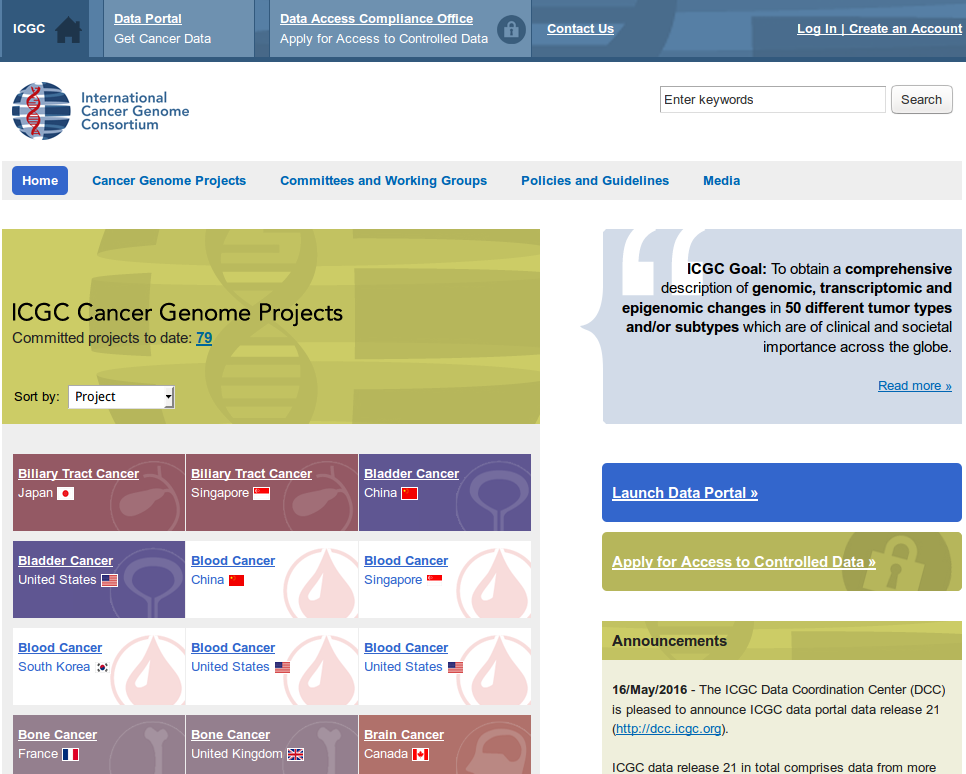
\includegraphics[width=0.8\textwidth]{c2_genomics/db_icgc_01.png}
  \end{figure}
\end{frame}

\begin{frame}
  \frametitle{NGS | 数据库 | ICGC}
  \begin{figure}
    \centering
    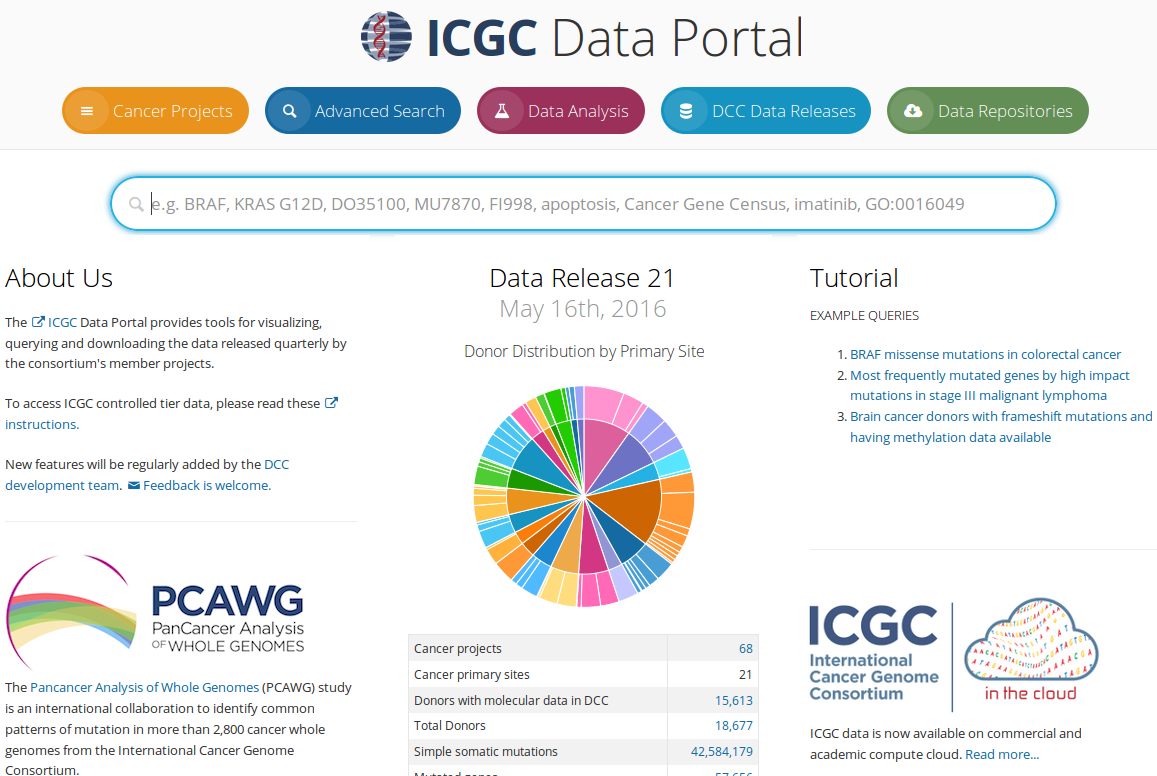
\includegraphics[width=0.9\textwidth]{c2_genomics/db_icgc_02.png}
  \end{figure}
\end{frame}

\begin{frame}
  \frametitle{NGS | 数据库 | GTEx}
  \begin{figure}
    \centering
    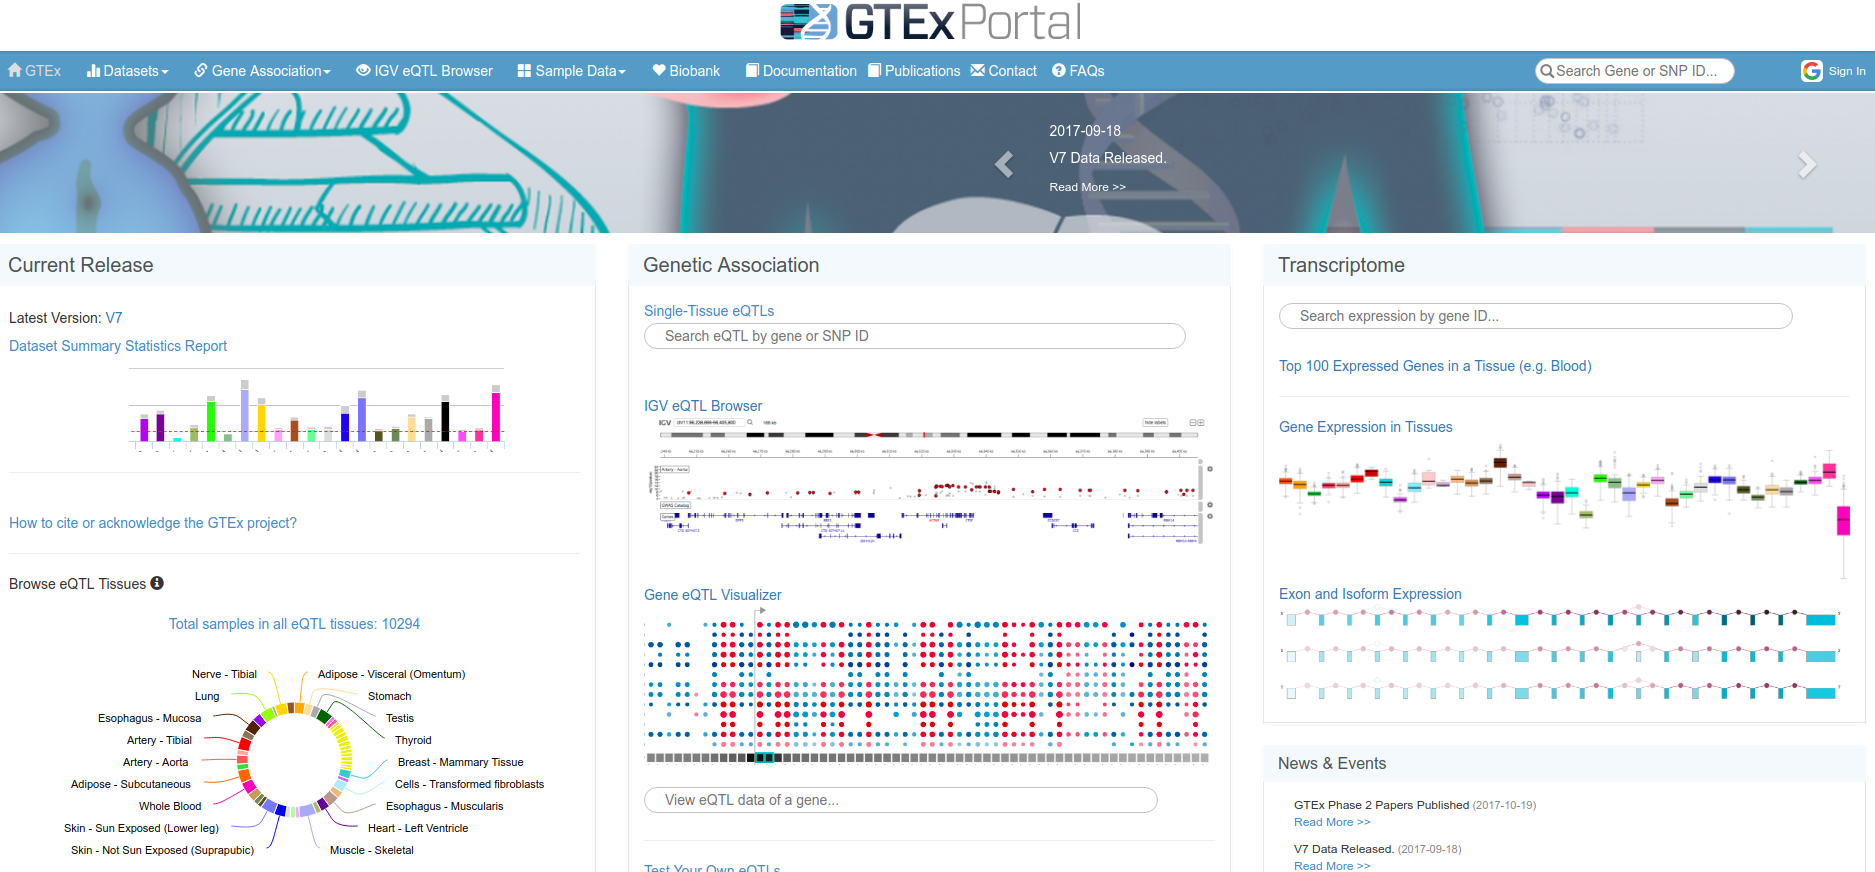
\includegraphics[width=\textwidth]{c2_genomics/db_gtex_01.png}
  \end{figure}
\end{frame}

\subsubsection{数据格式}
\begin{frame}
  \frametitle{NGS | 数据格式 | 概览}
  \begin{figure}
    \centering
    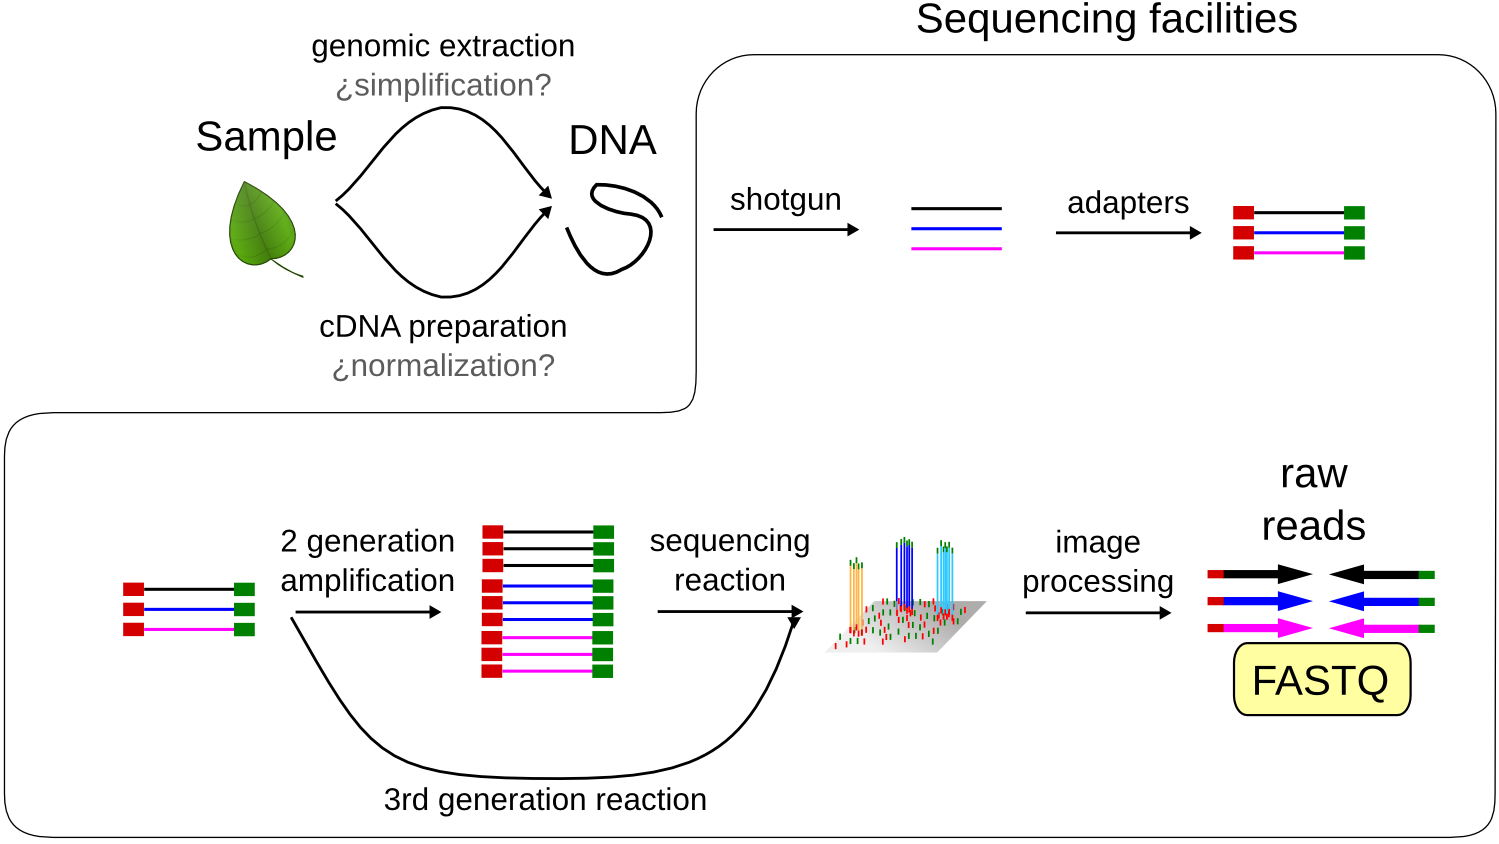
\includegraphics[width=0.9\textwidth]{c2_genomics/workflow_ngs_01.png}
  \end{figure}
\end{frame}

\begin{frame}
  \frametitle{NGS | 数据格式 | 概览}
  \begin{figure}
    \centering
    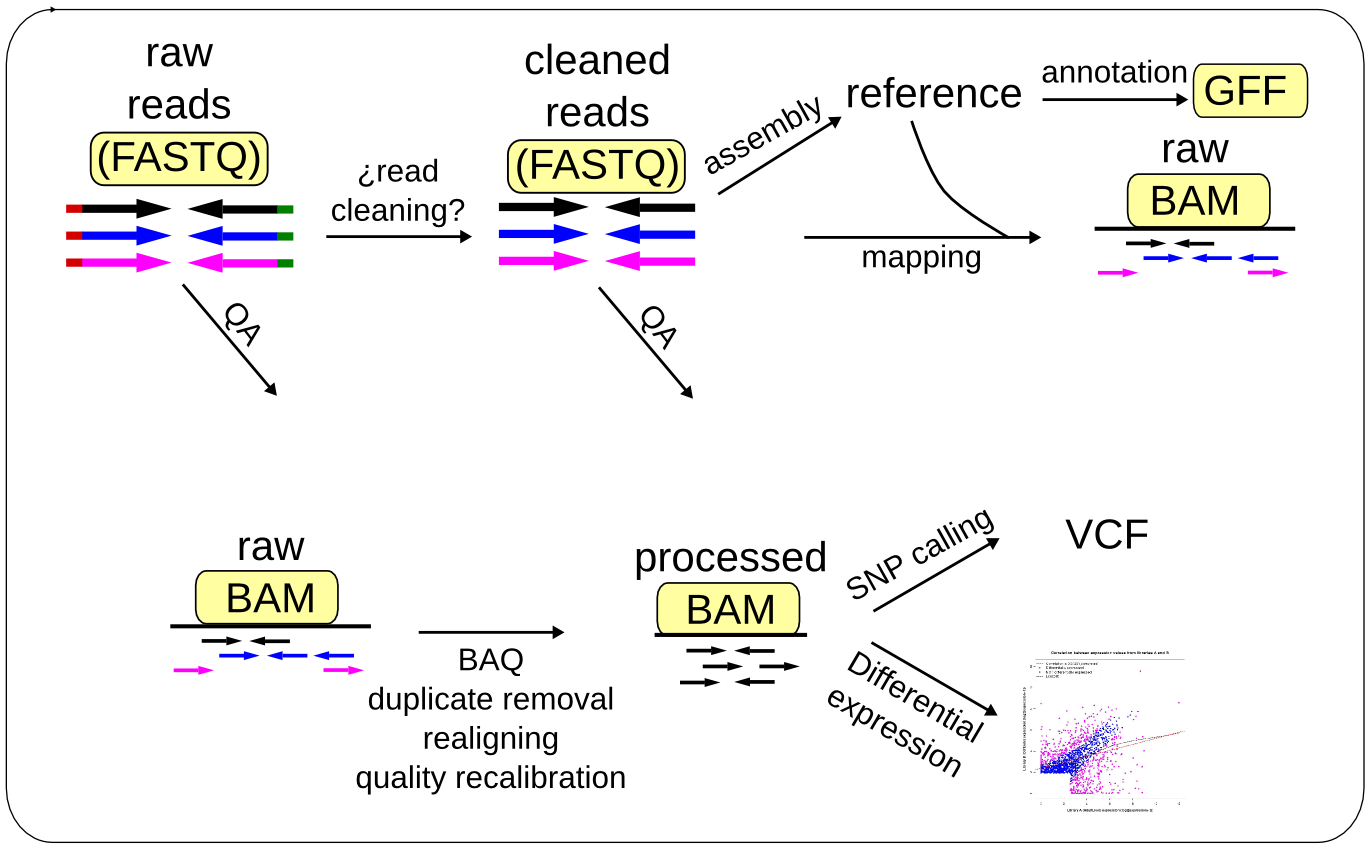
\includegraphics[width=0.9\textwidth]{c2_genomics/workflow_ngs_02.png}
  \end{figure}
\end{frame}

\begin{frame}
  \frametitle{NGS | 数据格式 | 简介}
  \begin{figure}
    \centering
    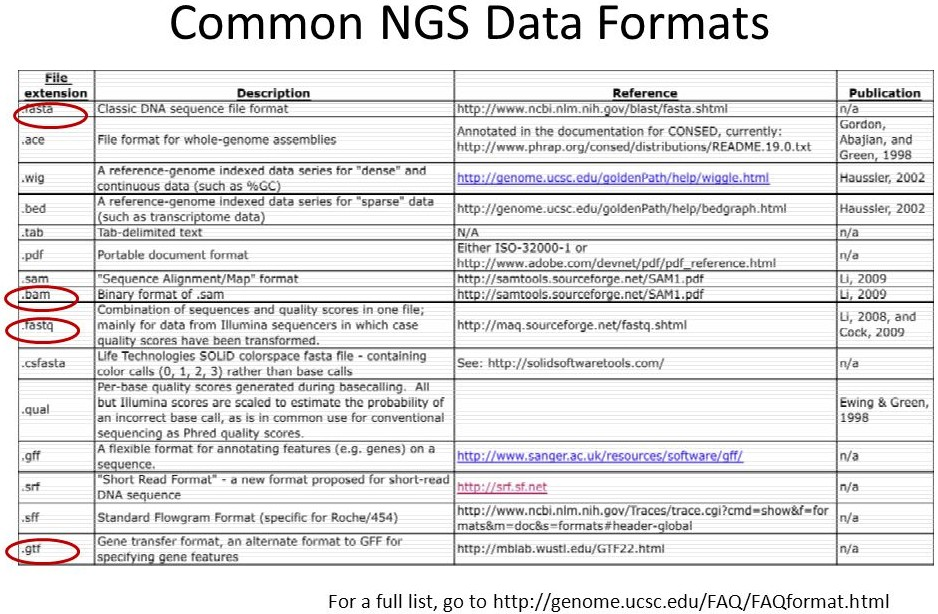
\includegraphics[width=0.9\textwidth]{c2_genomics/format_list_01.jpg}
  \end{figure}
\end{frame}

\begin{frame}
  \frametitle{NGS | 数据格式 | 简介}
  \begin{figure}
    \centering
    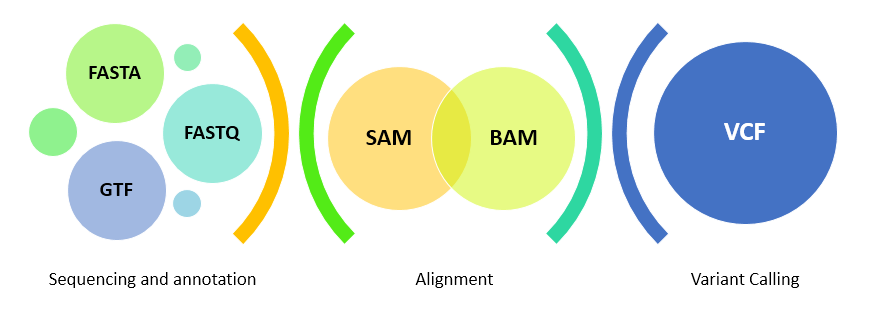
\includegraphics[width=0.9\textwidth]{c2_genomics/format_list_02.png}
  \end{figure}
\end{frame}

\begin{frame}
  \frametitle{NGS | 数据格式 | \textcolor{red}{简介}}
  \begin{block}{Reference sequences}
    \begin{itemize}
      \item FASTA
      \item 2bit
    \end{itemize}
  \end{block}
  \pause
  \begin{block}{Reads}
    \begin{itemize}
      \item FASTQ (FASTA with quality scores)
    \end{itemize}
  \end{block}
  \pause
  \begin{block}{Alignments}
    \begin{itemize}
      \item SAM (Sequence Alignment/Map format)
      \item BAM (Binary version of SAM)
    \end{itemize}
  \end{block}
\end{frame}

\begin{frame}
  \frametitle{NGS | 数据格式 | \textcolor{red}{简介}}
  \begin{block}{Features, annotation, coverage, scores}
    \begin{itemize}
      \item GFF3/GTF (General Feature Format, Gene Transfer Format)
      \item BED/bigBed (Browser Extensible Data)
      \item WIG/bigWig (Wiggle format)
      \item bedGraph
    \end{itemize}
  \end{block}
  \pause
  \begin{block}{Variations}
    \begin{itemize}
      \item VCF (Variant Call Format)
      \item BCF (Binary version of VCF)
    \end{itemize}
  \end{block}
\end{frame}

\begin{frame}
  \frametitle{NGS | 数据格式 | \alert{FASTA}}
  \begin{figure}
    \centering
    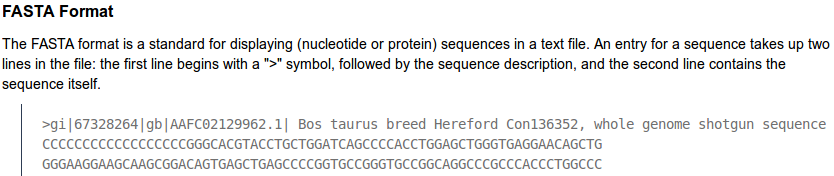
\includegraphics[width=0.9\textwidth]{c2_genomics/format_fasta_05.png}\\
    \vspace{1em}
    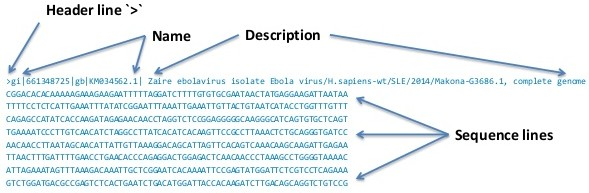
\includegraphics[width=0.9\textwidth]{c2_genomics/format_fasta_01.jpg}
  \end{figure}
\end{frame}

\begin{frame}
  \frametitle{NGS | 数据格式 | \alert{FASTQ}}
  \begin{figure}
    \centering
    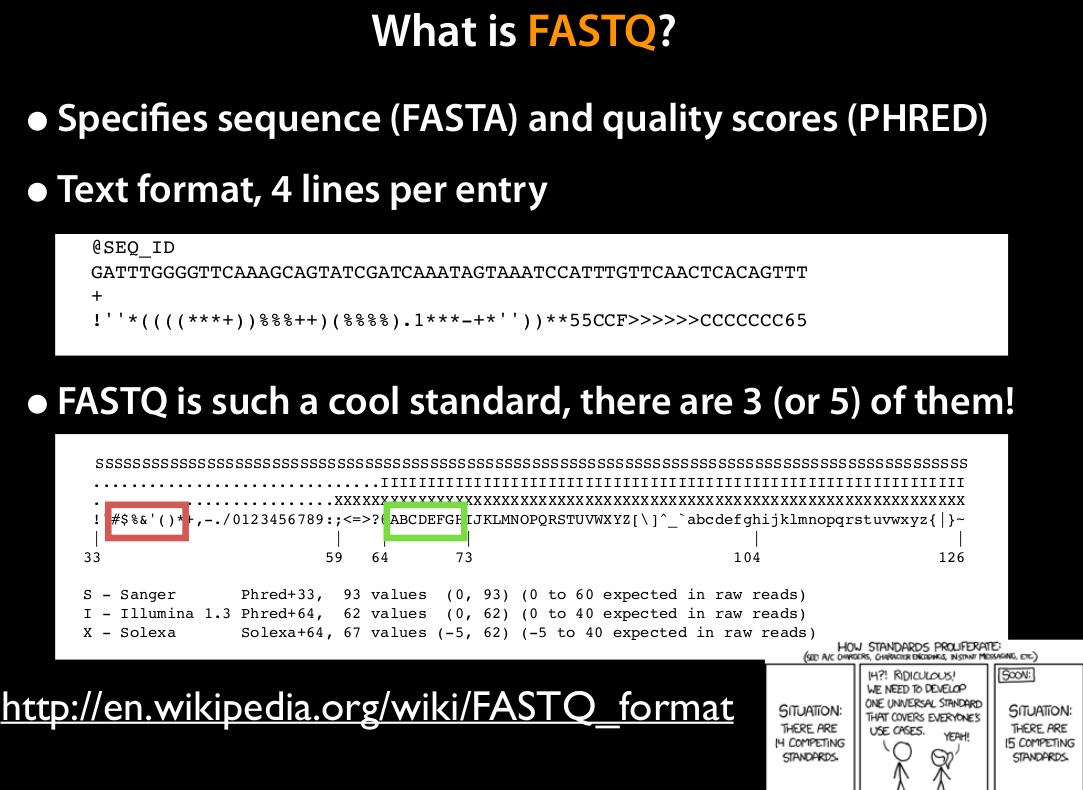
\includegraphics[width=0.9\textwidth]{c2_genomics/format_fastq_00.png}
  \end{figure}
\end{frame}

\begin{frame}
  \frametitle{NGS | 数据格式 | \alert{FASTQ}}
  \begin{figure}
    \centering
    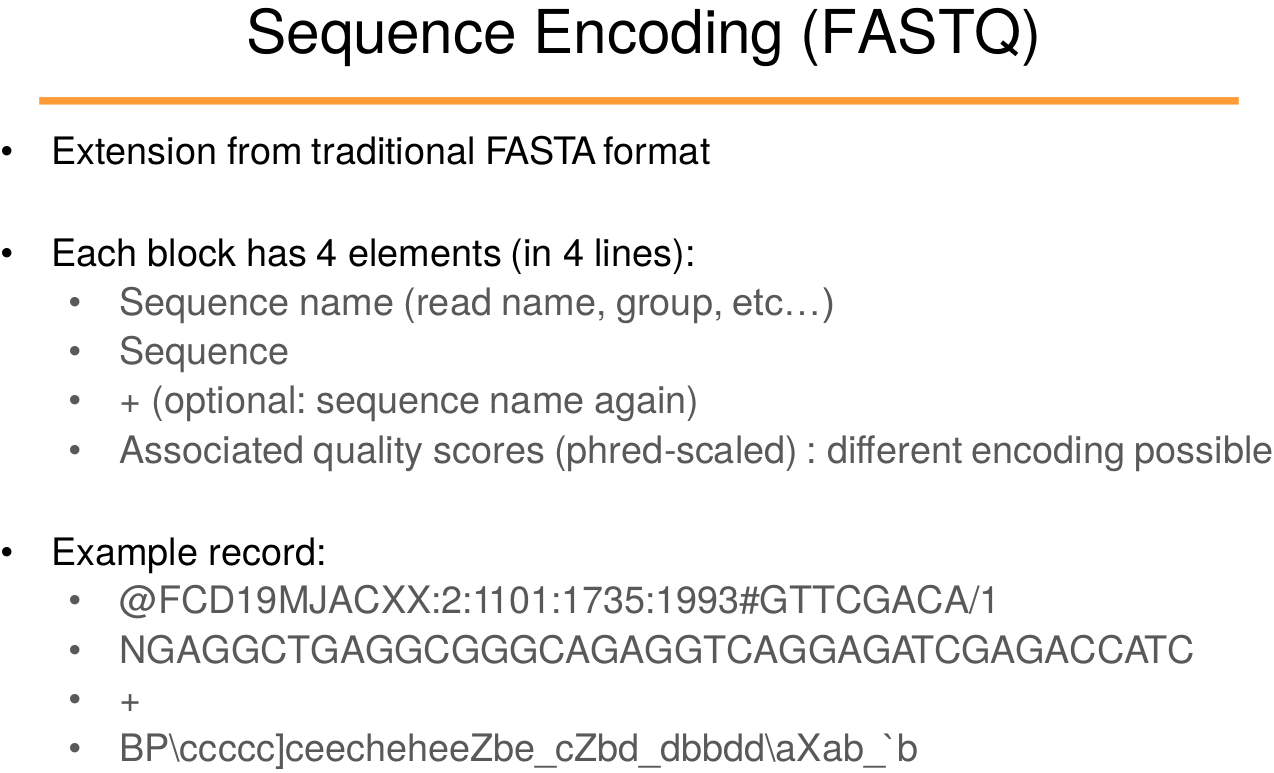
\includegraphics[width=\textwidth]{c2_genomics/format_fastq_06.png}
  \end{figure}
\end{frame}

\begin{frame}
  \frametitle{NGS | 数据格式 | FASTQ | ID | Illumina}
  \begin{figure}
    \centering
    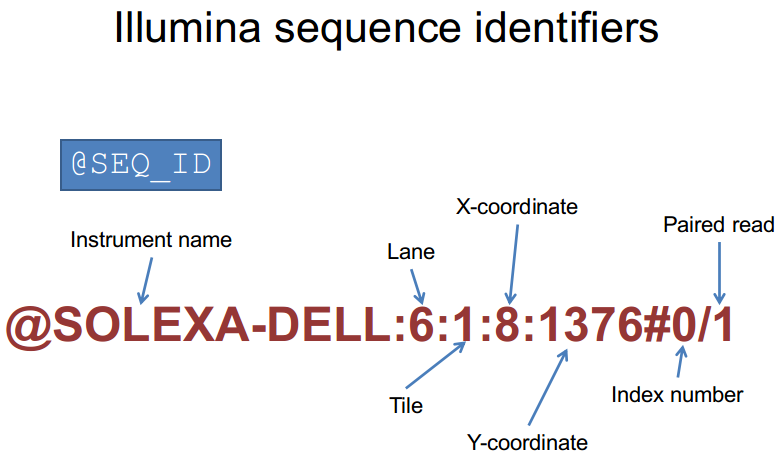
\includegraphics[width=0.9\textwidth]{c2_genomics/format_fastq_id_01.png}
  \end{figure}
\end{frame}

\begin{frame}
  \frametitle{NGS | 数据格式 | FASTQ | SRA}
  \begin{figure}
    \centering
    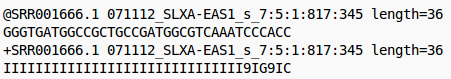
\includegraphics[width=0.9\textwidth]{c2_genomics/format_fastq_sra_02.png}
  \end{figure}
  \begin{block}{Note}
    \begin{itemize}
      \item ID = NCBI-assigned identifier + the original identifier from Solexa/Illumina + the read length
      \item \alert{fastq-dump}: lost the paired-end information, concatenate sequence of the forward and reverse reads together into a non-sense
      \item NCBI have converted this FASTQ data from the original Solexa/Illumina encoding to the \alert{Sanger standard}
    \end{itemize}
  \end{block}
\end{frame}

\begin{frame}
  \frametitle{NGS | 数据格式 | FASTQ | Quality | \textcolor{red}{Phred}}
  \begin{block}{Phred quality score}
A quality value Q is an integer mapping of p (i.e., the probability that the corresponding base call is incorrect).\\
\vspace{1em}
Phred quality score (the standard Sanger variant, assess reliability of a base call):
  \end{block}
  \begin{figure}
    \centering
    
\includegraphics[width=0.5\textwidth]{c2_genomics/format_fastq_qual_01.png}\\
    \vspace{1em}
    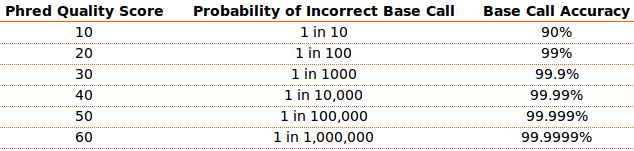
\includegraphics[width=0.8\textwidth]{c2_genomics/format_fastq_qual_02.png}
  \end{figure}
\end{frame}

\begin{frame}
  \frametitle{NGS | 数据格式 | FASTQ | Quality | Encoding}
  \begin{figure}
    \centering
    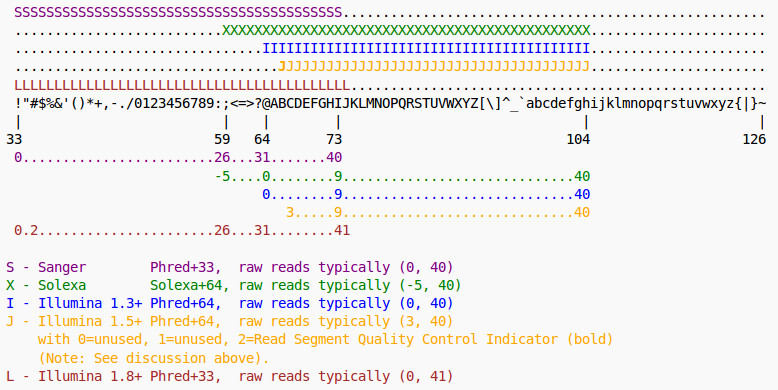
\includegraphics[width=\textwidth]{c2_genomics/format_fastq_qual_04.png}
  \end{figure}
\end{frame}

\begin{frame}
  \frametitle{NGS | 数据格式 | FASTQ | 用途}
  \begin{block}{Quality control}
    \begin{itemize}
      \item quality score distribution
      \item GC content
      \item k-mer enrichment
      \item ...
    \end{itemize}
  \end{block}
  \pause
  \begin{block}{Preprocessing}
    \begin{itemize}
      \item adapter removal
      \item low-quality reads filtering
      \item ...
    \end{itemize}
  \end{block}
  \pause
  \begin{block}{Processing}
    \begin{itemize}
      \item alignment
      \item further analysis
    \end{itemize}
  \end{block}
\end{frame}

\begin{frame}
  \frametitle{NGS | 数据格式 | SAM}
  \begin{figure}
    \centering
    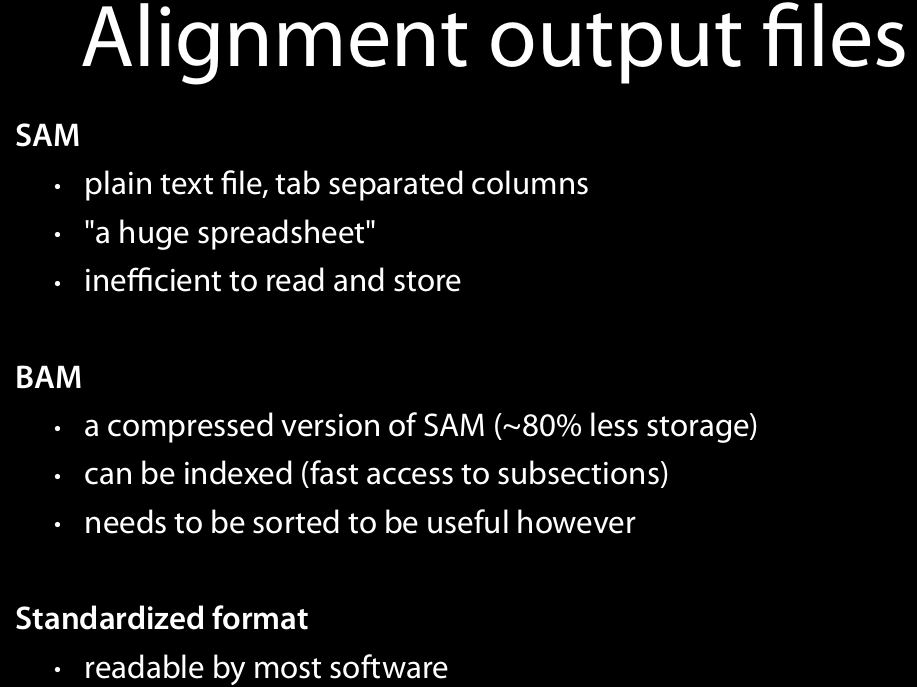
\includegraphics[width=0.85\textwidth]{c2_genomics/format_sam_30.png}
  \end{figure}
\end{frame}

\begin{frame}
  \frametitle{NGS | 数据格式 | SAM}
  \begin{figure}
    \centering
    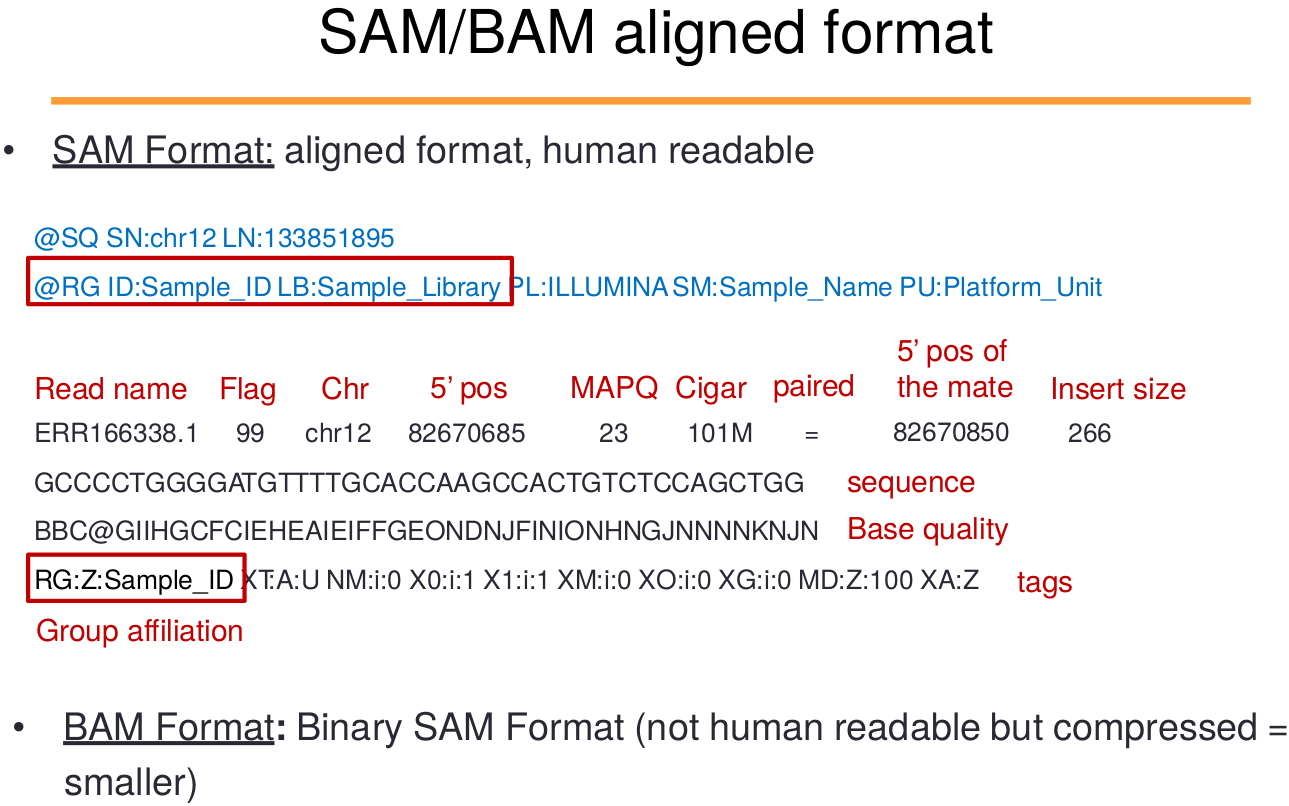
\includegraphics[width=0.8\textwidth]{c2_genomics/format_sam_32.png}
  \end{figure}
  \vspace{-0.8em}
  \begin{block}{SAM Format Specification}
    \href{https://samtools.github.io/hts-specs/SAMv1.pdf}{https://samtools.github.io/hts-specs/SAMv1.pdf}
  \end{block}
\end{frame}

\begin{frame}
  \frametitle{NGS | 数据格式 | \textcolor{red}{SAM}}
  \begin{figure}
    \centering
    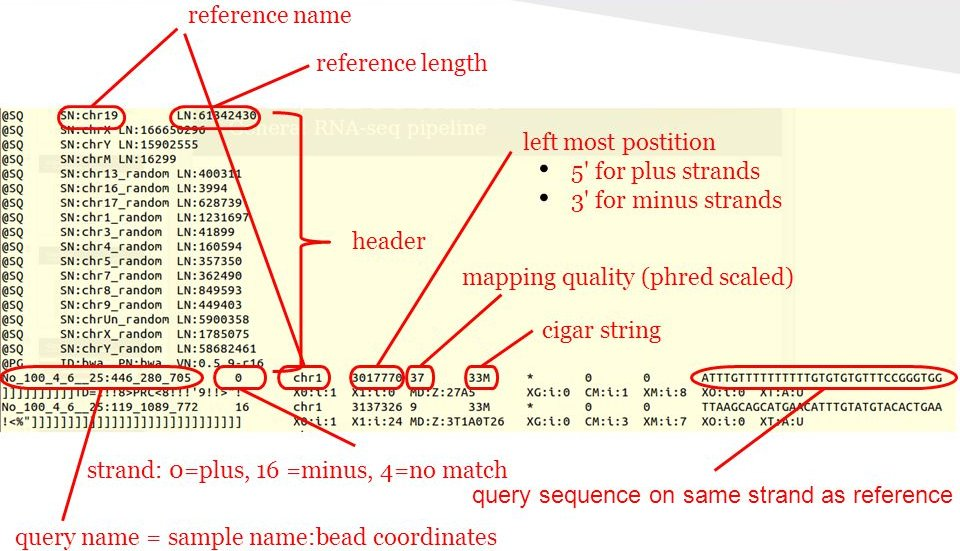
\includegraphics[width=0.95\textwidth]{c2_genomics/format_sam_06.jpg}
  \end{figure}
\end{frame}

\begin{frame}
  \frametitle{NGS | 数据格式 | SAM}
  \begin{figure}
    \centering
    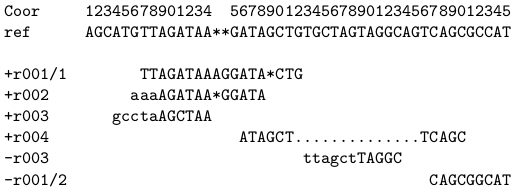
\includegraphics[width=0.6\textwidth]{c2_genomics/format_sam_03.png}\\
    \vspace{1em}
    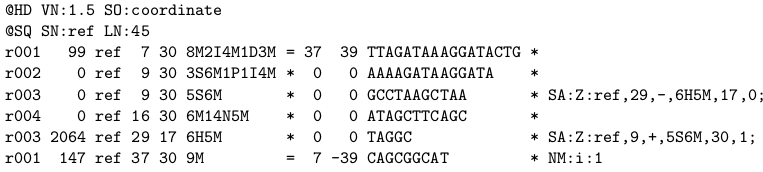
\includegraphics[width=0.9\textwidth]{c2_genomics/format_sam_04.png}
  \end{figure}
\end{frame}

\begin{frame}
  \frametitle{NGS | 数据格式 | BAM}
  \begin{figure}
    \centering
    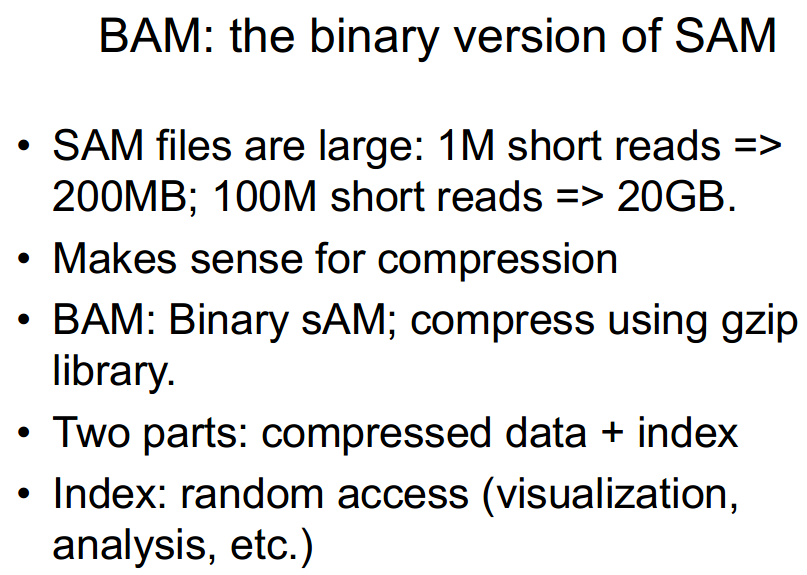
\includegraphics[width=0.8\textwidth]{c2_genomics/format_bam_01.png}
  \end{figure}
\end{frame}

\begin{frame}
  \frametitle{NGS | 数据格式 | \textcolor{red}{BED}}
  \begin{figure}
    \centering
    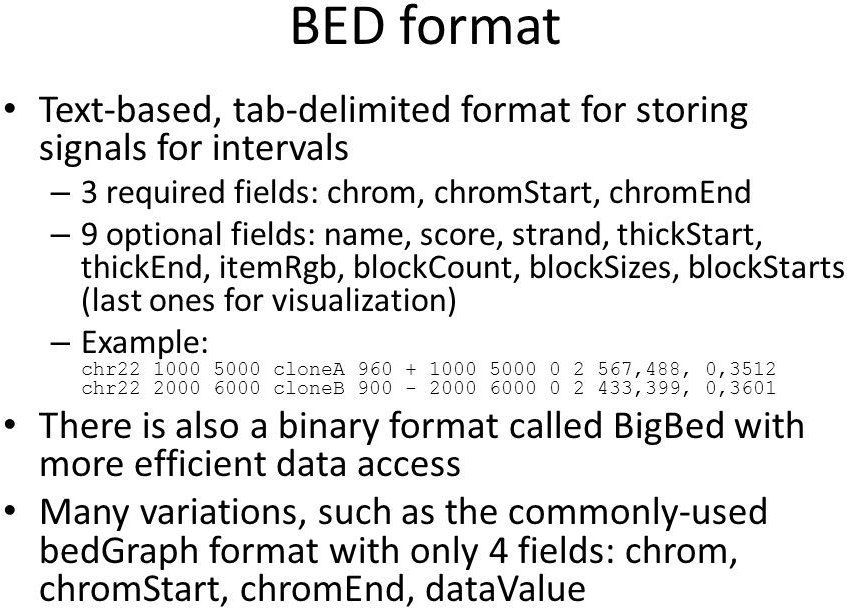
\includegraphics[width=0.9\textwidth]{c2_genomics/format_bed_01.jpg}
  \end{figure}
\end{frame}

\begin{frame}
  \frametitle{NGS | 数据格式 | BED}
  \begin{figure}
    \centering
    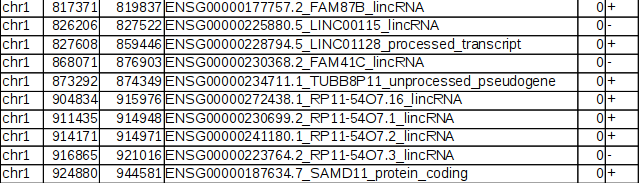
\includegraphics[width=\textwidth]{c2_genomics/format_bed_10.png}
  \end{figure}
\end{frame}

\begin{frame}
  \frametitle{NGS | 数据格式 | GTF/GFF}
  \begin{figure}
    \centering
    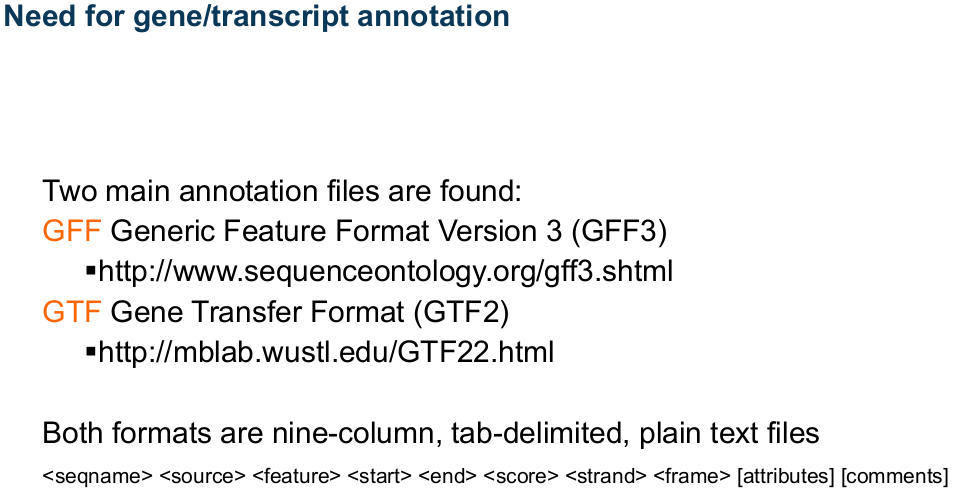
\includegraphics[width=0.9\textwidth]{c2_genomics/format_gtf_gff_02.png}
  \end{figure}
\end{frame}

\begin{frame}
  \frametitle{NGS | 数据格式 | GTF}
  \begin{figure}
    \centering
    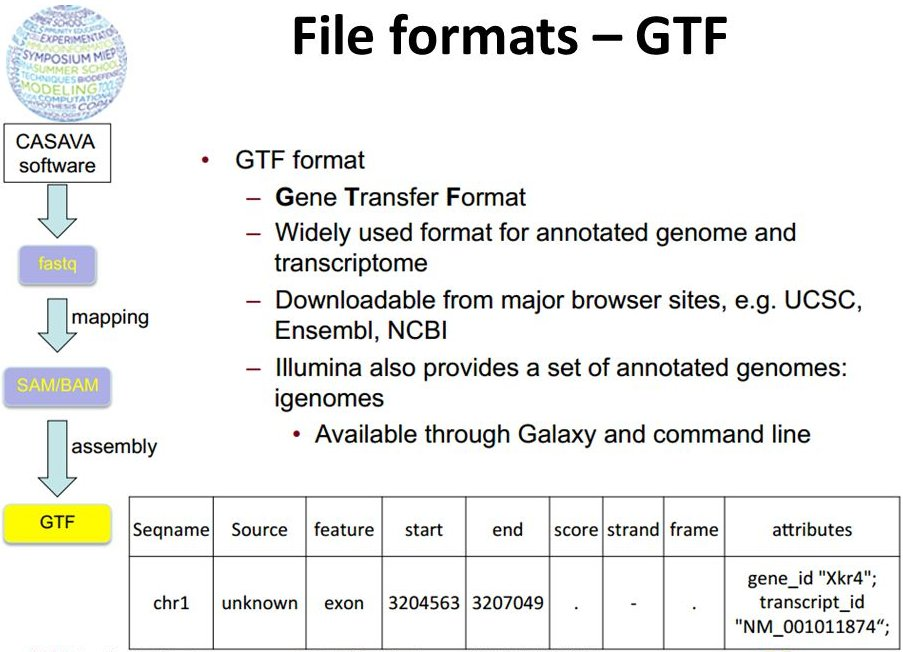
\includegraphics[width=0.9\textwidth]{c2_genomics/format_gtf_01.jpg}
  \end{figure}
\end{frame}

\begin{frame}
  \frametitle{NGS | 数据格式 | GTF}
  \begin{figure}
    \centering
    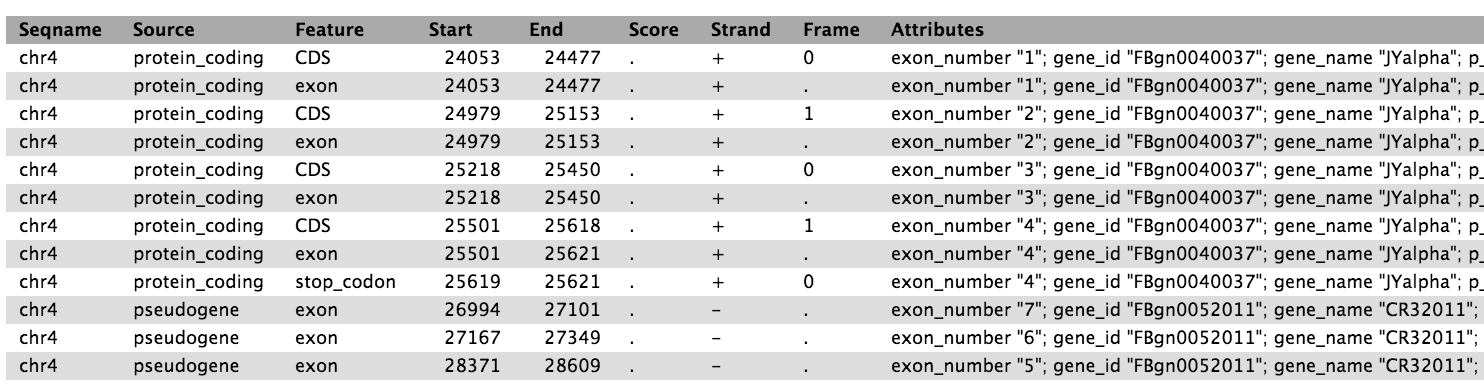
\includegraphics[width=\textwidth]{c2_genomics/format_gtf_10.png}
  \end{figure}
\end{frame}

\begin{frame}
  \frametitle{NGS | 数据格式 | \textcolor{red}{GFF}}
  \begin{figure}
    \centering
    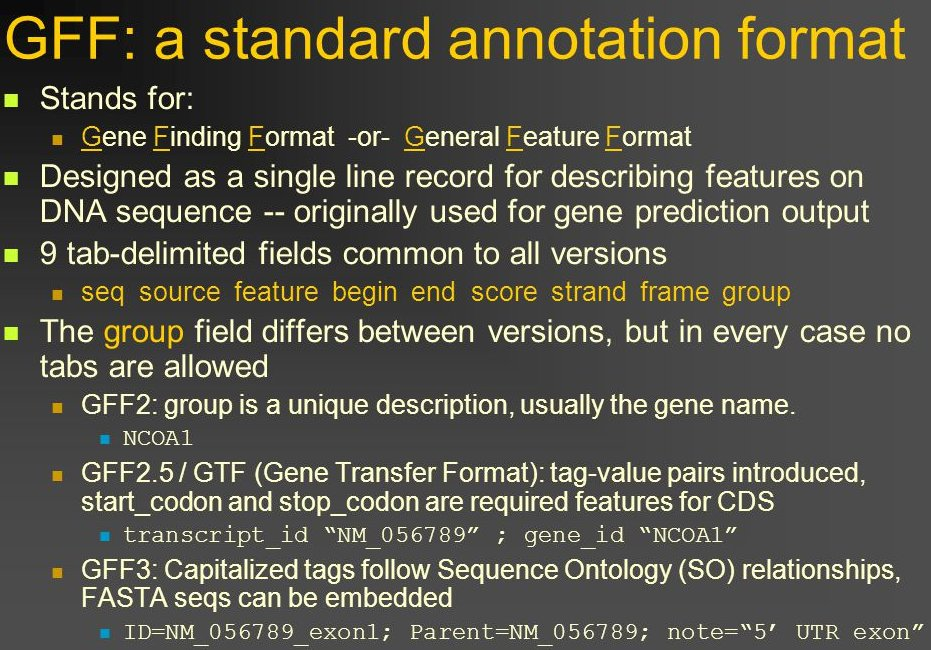
\includegraphics[width=0.9\textwidth]{c2_genomics/format_gff_01.jpg}
  \end{figure}
\end{frame}

\begin{frame}
  \frametitle{NGS | 数据格式 | GFF}
  \begin{figure}
    \centering
    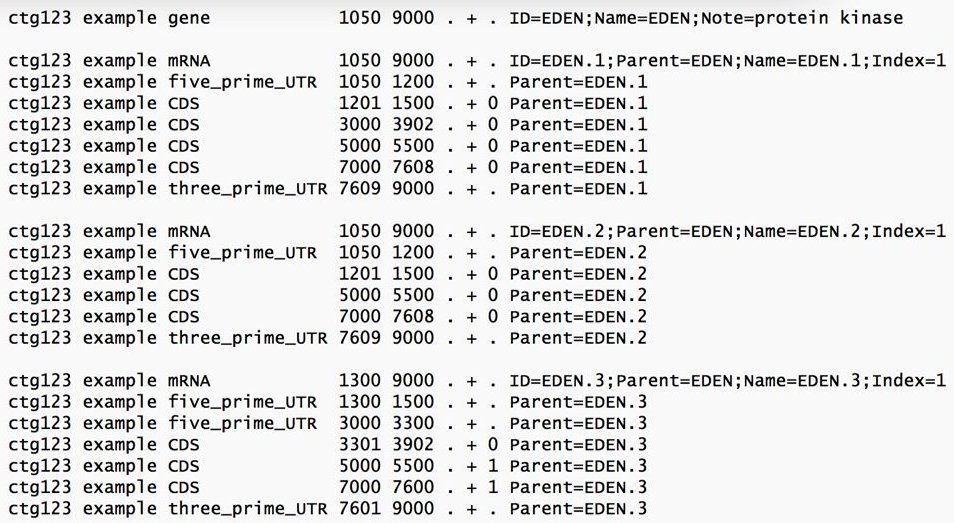
\includegraphics[width=\textwidth]{c2_genomics/format_gff_10.jpg}
  \end{figure}
\end{frame}

\begin{frame}
  \frametitle{NGS | 数据格式 | GTF vs. GFF}
  \begin{figure}
    \centering
    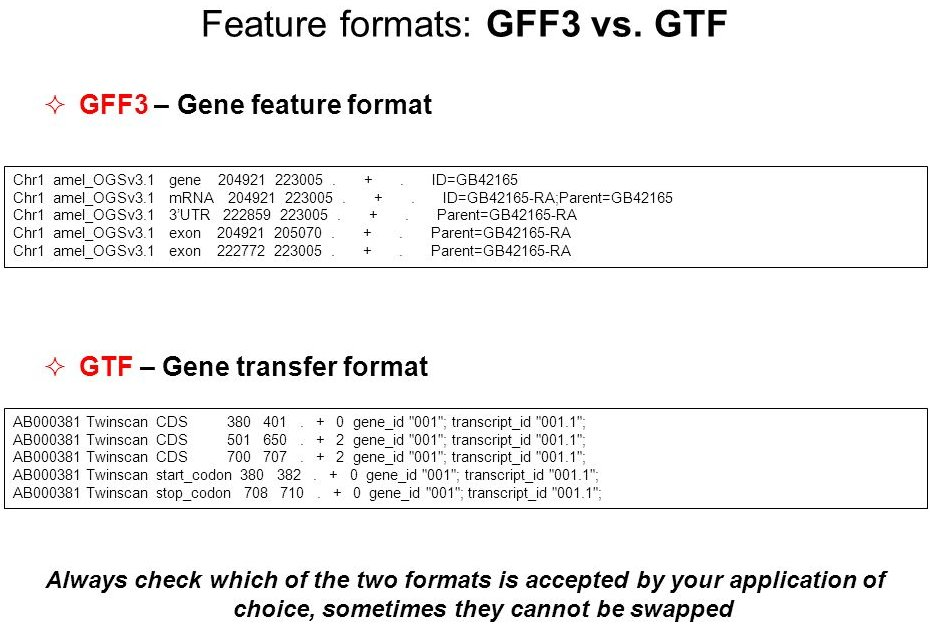
\includegraphics[width=0.9\textwidth]{c2_genomics/format_gtf_gff_01.jpg}
  \end{figure}
\end{frame}

\begin{frame}
  \frametitle{NGS | 数据格式 | GTF vs. GFF}
  \begin{figure}
    \centering
    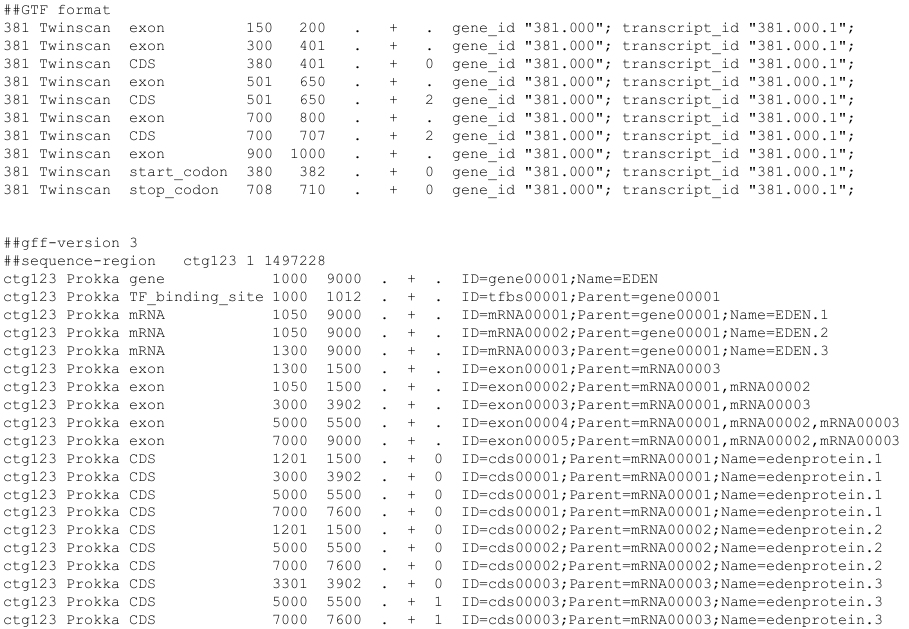
\includegraphics[width=0.9\textwidth]{c2_genomics/format_gtf_gff_03.png}
  \end{figure}
\end{frame}

\begin{frame}
  \frametitle{NGS | 数据格式 | \alert{BED vs. GFF}}
  \begin{figure}
    \centering
    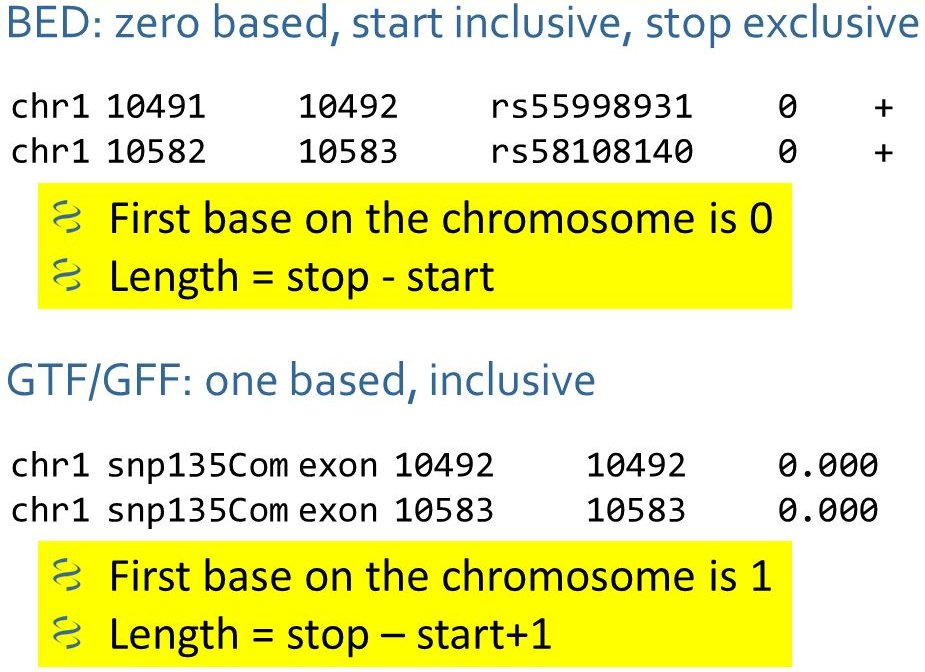
\includegraphics[width=0.9\textwidth]{c2_genomics/format_bed_gff_01.jpg}
  \end{figure}
\end{frame}

\begin{frame}
  \frametitle{NGS | 数据格式 | BED vs. GFF}
  \begin{figure}
    \centering
    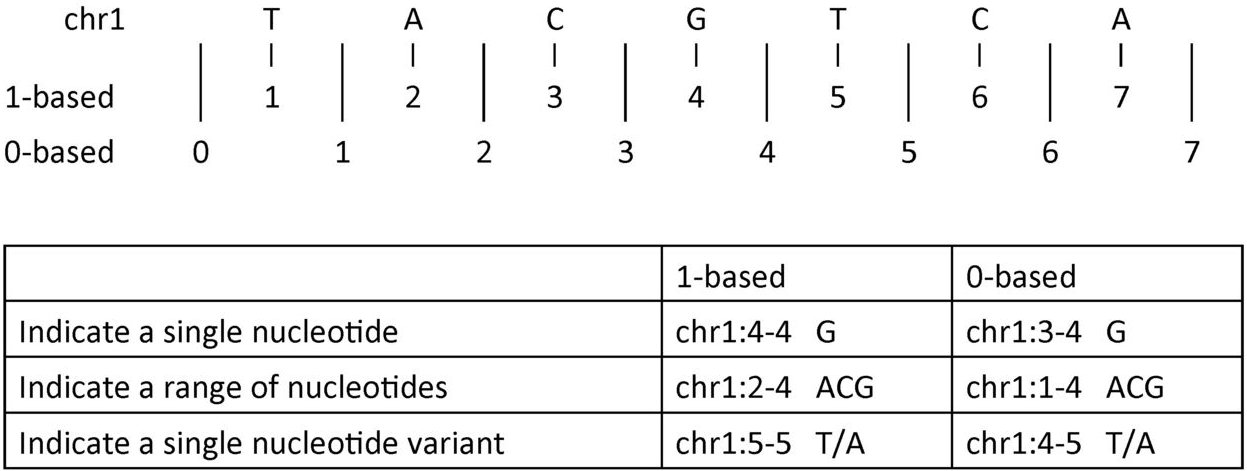
\includegraphics[width=\textwidth]{c2_genomics/format_bed_gff_02.jpg}
  \end{figure}
\end{frame}

\begin{frame}
  \frametitle{NGS | 数据格式 | VCF}
  \begin{figure}
    \centering
    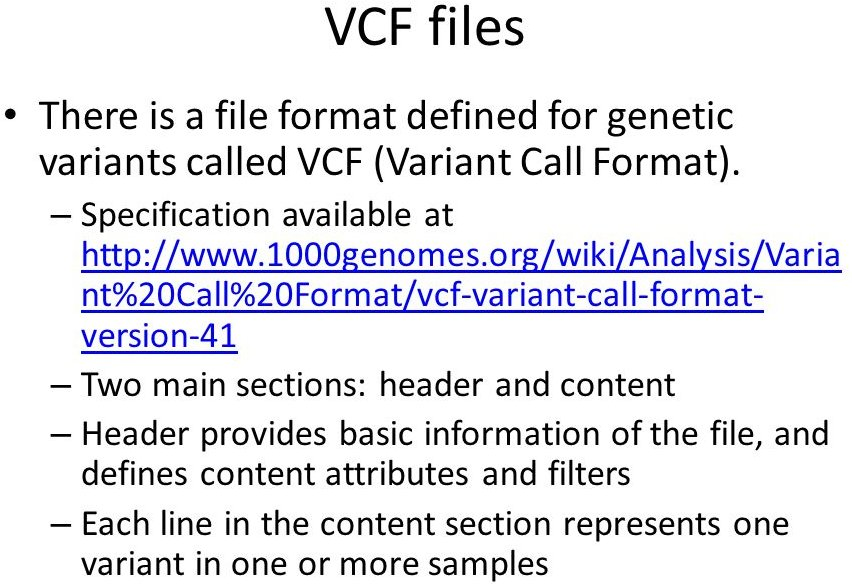
\includegraphics[width=0.9\textwidth]{c2_genomics/format_vcf_01.jpg}
  \end{figure}
\end{frame}

\begin{frame}
  \frametitle{NGS | 数据格式 | \alert{VCF}}
  \begin{figure}
    \centering
    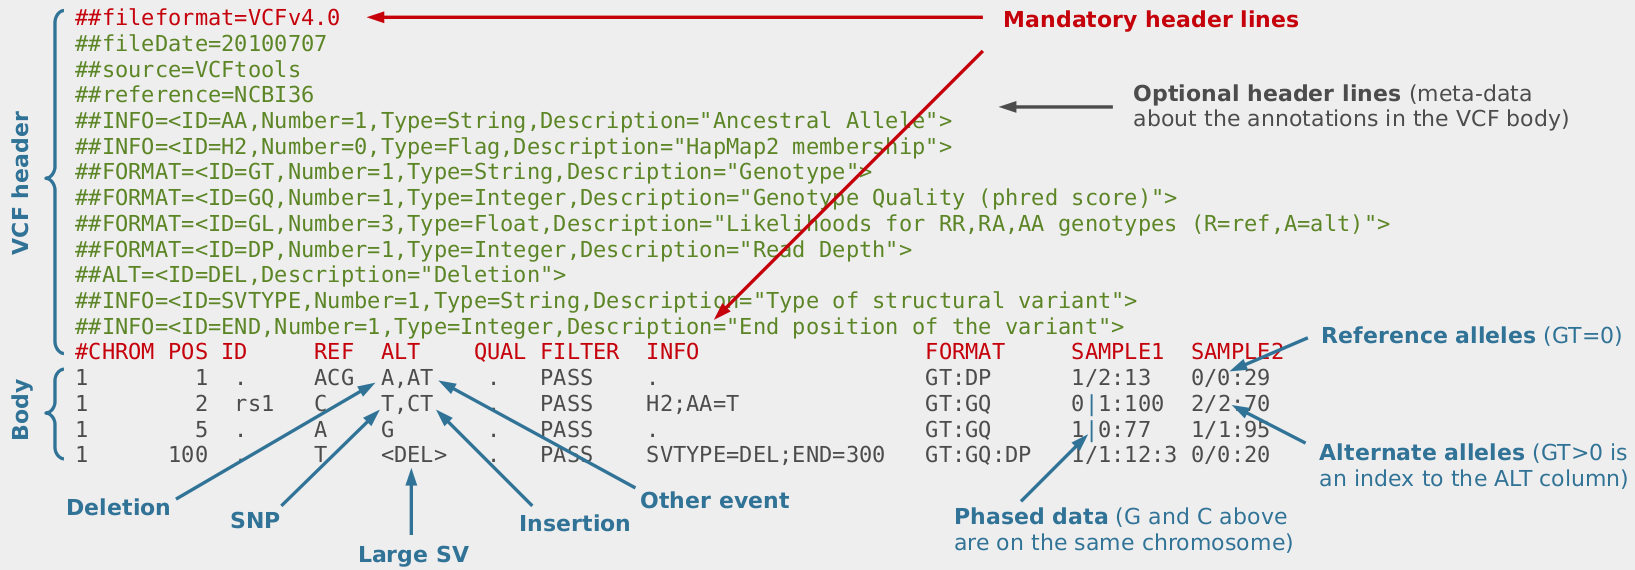
\includegraphics[width=\textwidth]{c2_genomics/format_vcf_05.png}
  \end{figure}
\end{frame}

